\documentclass[12pt,a4paper]{article}
\usepackage[utf8]{inputenc}
\usepackage{amsmath, amssymb, amsfonts}
\usepackage{graphicx}
\usepackage{float}
\usepackage{geometry}
\geometry{margin=2.5cm}

\title{Diskretna fourierova analiza}
\author{Filip Jesenšek (28231064)}
\date{\today}

\begin{document}

\maketitle

\begin{abstract}
V tem poročilu obravnavamo numerično izračunavanje Fourierove transformacije diskretnih signalov. Izvedli smo analizo preprostih sintetičnih vzorcev in opazovali pojav potujitve (aliasing) pri prekoračitvi Nyquistove frekvence. Podrobno smo analizirali numerično natančnost lastne implementacije DFT v primerjavi z NumPy FFT ter preverili reverzibilnost z inverzno transformacijo. V drugem delu smo analizirali vzorce začetka Bachove partite za violino solo pri šestih različnih frekvencah vzorčenja (44.1 kHz, 11.025 kHz, 5.512 kHz, 2.756 kHz, 1.378 kHz in 882 Hz) ter s pomočjo Fourierovega spektra in poslušanja .mp3 datotek ugotavljali vpliv zniževanja vzorčne frekvence. Rezultate smo prikazali z več različnimi vizualizacijami (posamezni spektri, primerjava z navpičnim zamikom, normirani spekter, logaritemski prikaz in 3D waterfall diagram) ter potrdili prisotnost ali odsotnost potujitve.
\end{abstract}

\section{Uvod}
Fourierova analiza je temeljno orodje za obdelavo signalov, saj omogoča prehod iz časovne v frekvenčno domeno. V praksi običajno nimamo zveznega signala, temveč diskretne vzorce \(h_k = h(t_k)\) z enakomernim razmikom \(\Delta\). V skladu z nalogo nas zanima numerično računanje diskretne Fourierove transformacije (DFT) in razumevanje pojava potujitve (aliasing), ko signal vsebuje frekvence nad Nyquistovo frekvenco \(f_c = 1/(2\Delta)\).

\section{Teoretične osnove}
Za vzorčeni signal \(h_k = h(k\Delta), k=0,1,\dots, N-1\) je diskretna Fourierova transformacija definirana kot:
\begin{equation}
H_n = \sum_{k=0}^{N-1} h_k \exp\left(2\pi i k n / N\right), \qquad n = -\frac{N}{2}, \dots, \frac{N}{2}.
\end{equation}
Povezava z zvezno Fourierovo transformacijo \(H(f)\) je podana s približkom \(H(n/(N\Delta)) \approx \Delta \cdot H_n\). Frekvenčna ločljivost je \(\Delta f = 1/(N\Delta)\), Nyquistova frekvenca pa \(f_c = 1/(2\Delta)\). Obratna transformacija je:
\begin{equation}
h_k = \frac{1}{N} \sum_{n=0}^{N-1} H_n \exp\left(-2\pi i k n / N\right).
\end{equation}
Pri realnih signalih velja simetrija \(H_{N-n} = H_n^*\), zato za enostransko spektralno gostoto moči (PSD) velja \(P_n = |H_n|^2 + |H_{N-n}|^2 = 2|H_n|^2\) za \(n \neq 0, N/2\). Parsevalov izrek povezuje energijo v časovni in frekvenčni domeni:
\begin{equation}
\sum_{k=0}^{N-1} |h_k|^2 = \frac{1}{N} \sum_{n=0}^{N-1} |H_n|^2.
\end{equation}

\section{Rezultati in analiza}

\subsection{Analiza sintetičnih vzorcev}
Najprej smo ustvarili časovni signal, sestavljen iz dveh sinusnih komponent: \(h(t) = \sin(2\pi f_1 t) + 0.5 \sin(2\pi f_2 t)\) z \(f_1 = 5\) Hz in \(f_2 = 20\) Hz. Vzorčili smo s frekvenco \(f_s = 1/\Delta = 10000\) Hz, pri čemer je \(N = 10000\). Nyquistova frekvenca je \(f_c = 5000\) Hz, kar pomeni, da sta obe frekvenci pod mejo in do potujitve ne pride.

Na sliki \ref{fig:periodic} je prikazan amplitudni spekter. Vidimo dva jasna vrhova pri 5 Hz in 20 Hz, kar se odlično ujema z vhodnima frekvencama.

\begin{figure}[H]
    \centering
    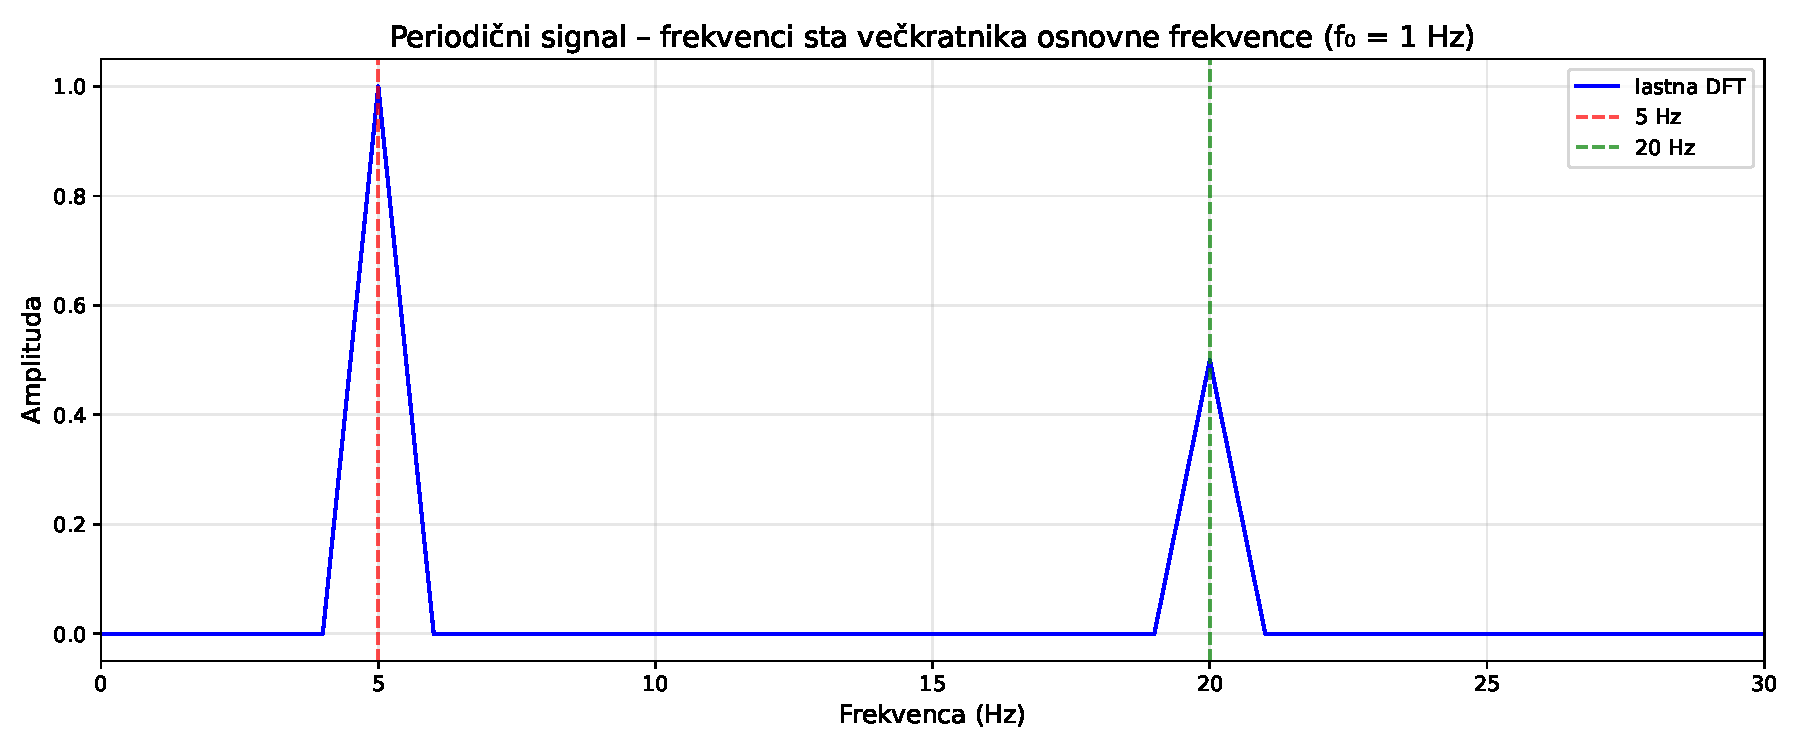
\includegraphics[width=0.8\textwidth]{periodic_spectrum.pdf}
    \caption{Amplitudni spekter periodičnega signala. Frekvenci (5 Hz in 20 Hz) sta celoštevilska večkratnika osnovne frekvence 1 Hz.}
    \label{fig:periodic}
\end{figure}

\subsection{Spektralno razlivanje (leakage)}
Ko signal v vzorčnem intervalu ni periodičen, pride do pojava spektralnega razlivanja. Na sliki \ref{fig:nonperiodic} smo uporabili frekvenci \(f_1 = 5.3\) Hz in \(f_2 = 20.7\) Hz, ki nista večkratnika osnovne frekvence \(f_0 = 1\) Hz. Opazimo, da se energija razlije v sosednje frekvenčne binove, vrhova pa nista več tako ostra kot pri periodičnem primeru.

\begin{figure}[H]
    \centering
    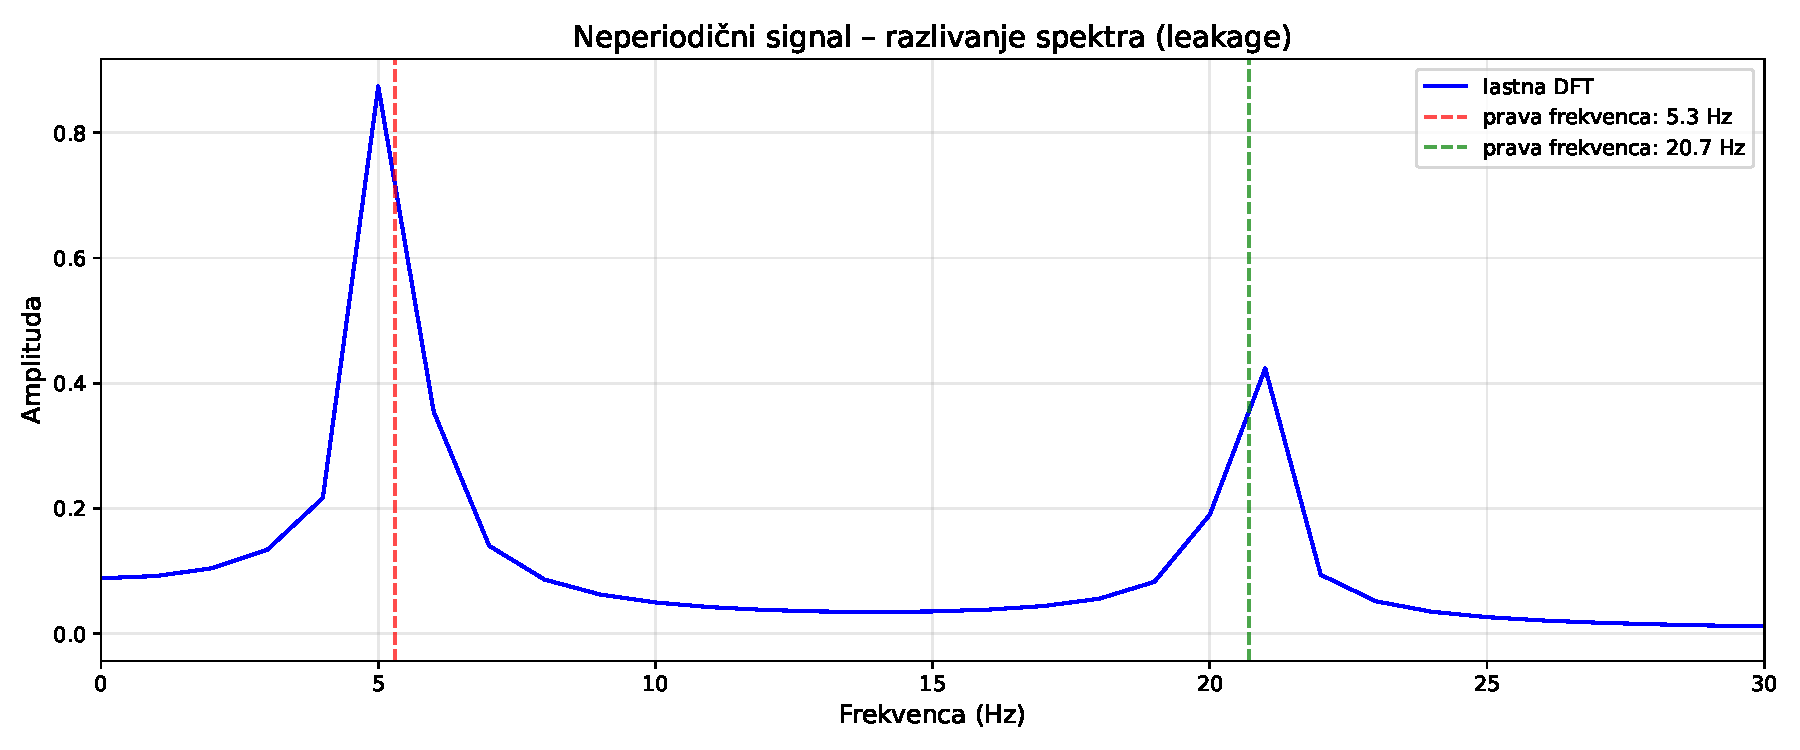
\includegraphics[width=0.8\textwidth]{nonperiodic_spectrum.pdf}
    \caption{Spektralno razlivanje pri neperiodičnem signalu. Energija se razlije v sosednje frekvenčne binove.}
    \label{fig:nonperiodic}
\end{figure}

\subsection{Pojav potujitve (aliasing)}
Da bi opazovali potujitev, smo uporabili signal \(h(t) = \sin(2\pi f_1 t) + \sin(2\pi f_2 t)\) s frekvencama \(f_1 = 10\) Hz in \(f_2 = 80\) Hz. Vzorčili smo s frekvenco \(f_s = 100\) Hz, zato je Nyquistova frekvenca \(f_c = 50\) Hz. Po izreku o vzorčenju se frekvenca \(f_2 = 80\) Hz preslika v \(f_{\text{aliased}} = f_s - f_2 = 20\) Hz.

\begin{figure}[H]
    \centering
    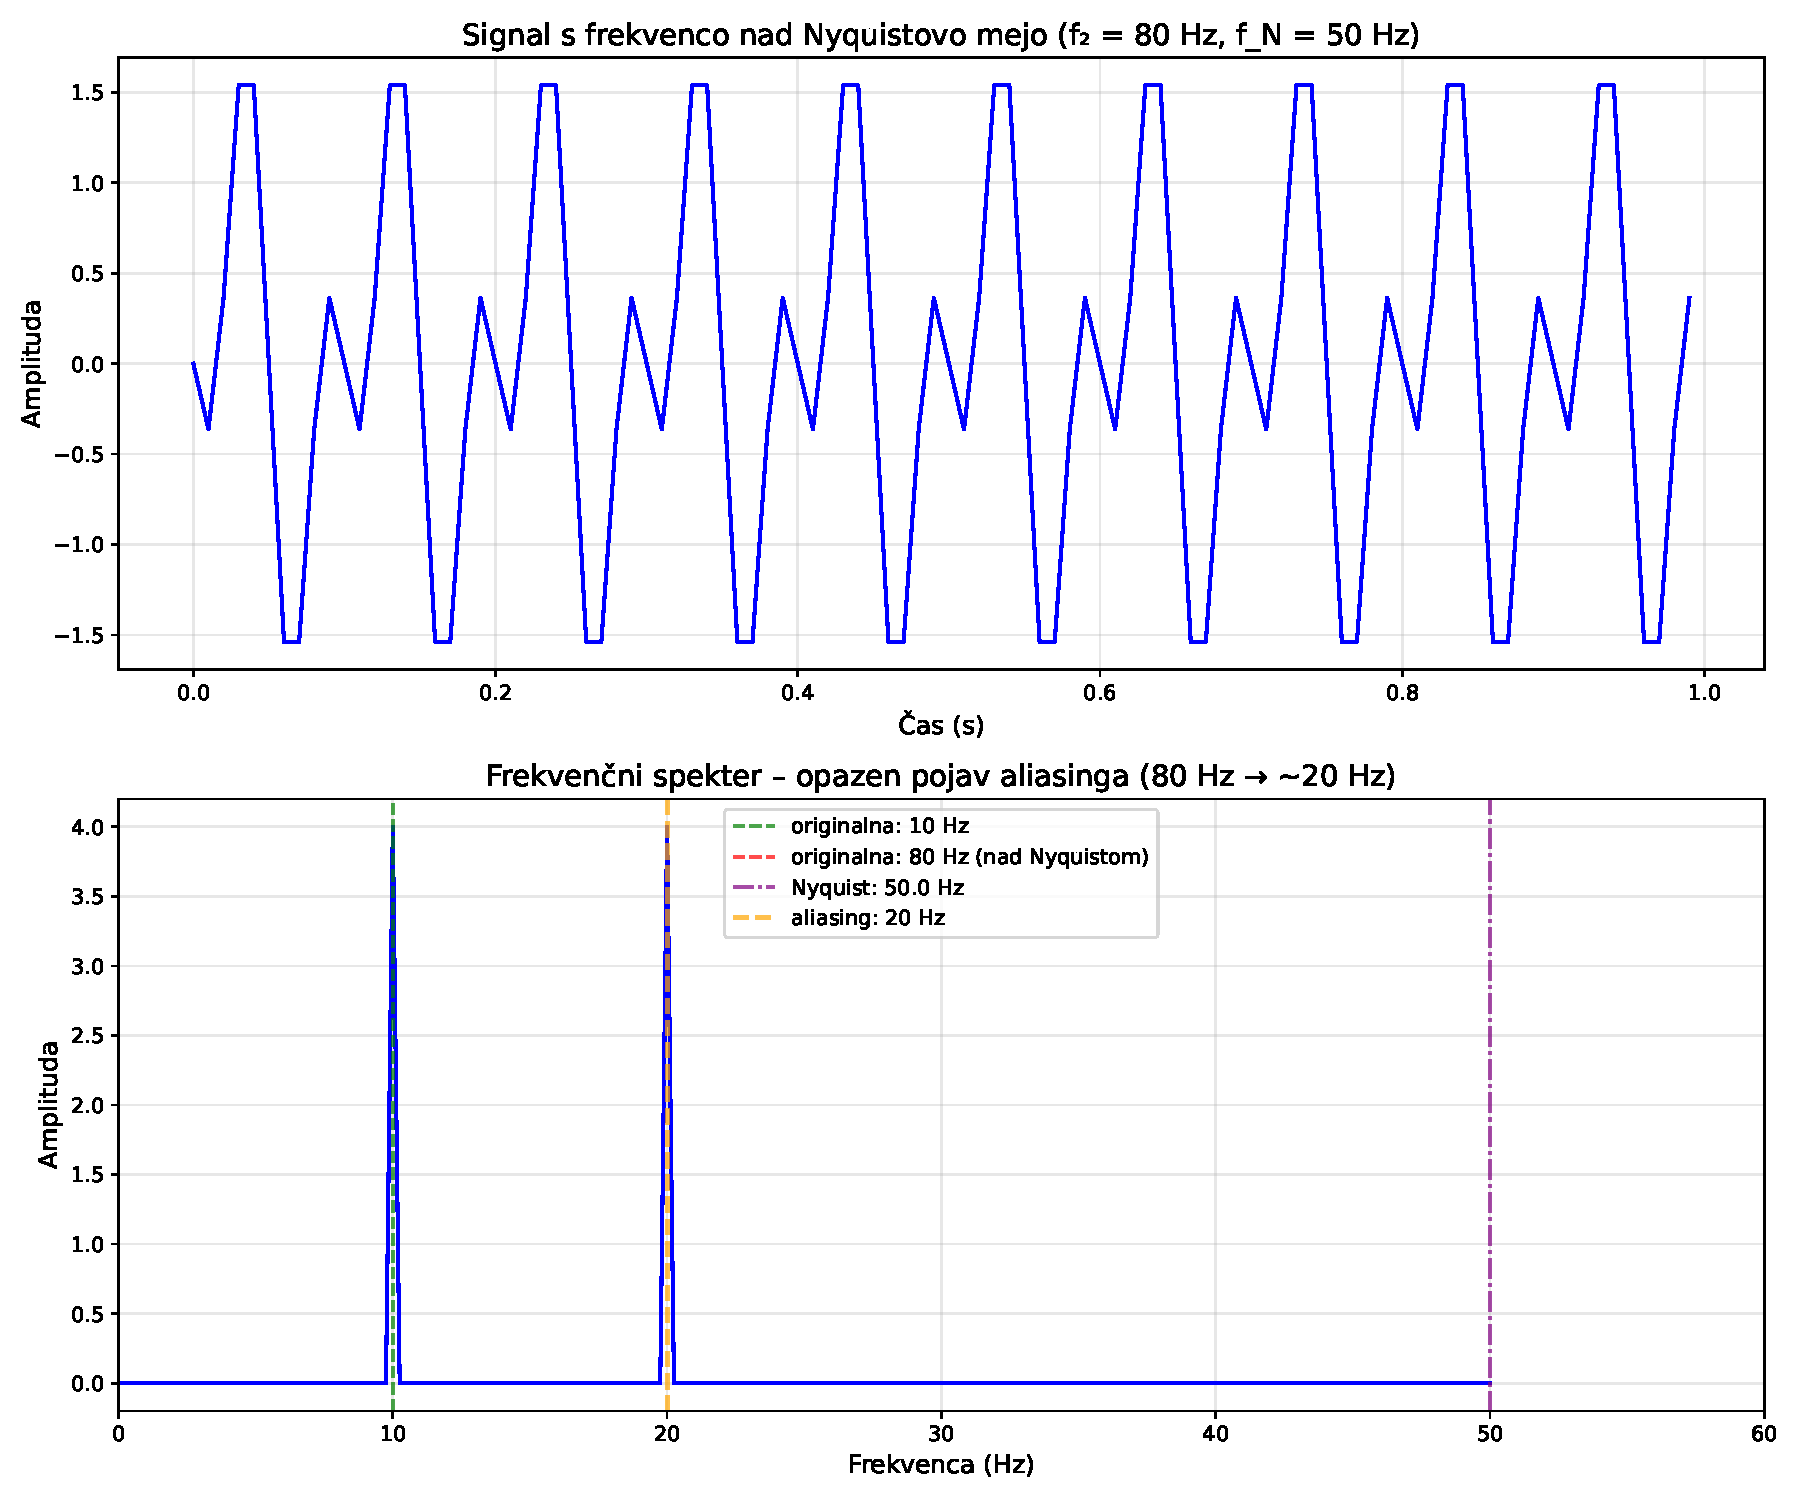
\includegraphics[width=0.8\textwidth]{aliasing_synthetic.pdf}
    \caption{Prikaz potujitve za signal z 80 Hz, vzorčen pri 100 Hz. V spektru se vrh pričakovano pojavi pri 20 Hz (aliasing), namesto pri 80 Hz.}
    \label{fig:aliasing}
\end{figure}

Na sliki \ref{fig:aliasing} je amplitudni spekter signala. Poleg vrha pri 10 Hz opazimo vrh pri \(f = 20\) Hz, kar je jasen dokaz potujitve. Frekvenca 80 Hz se je preslikala v 20 Hz.

\subsection{Numerična natančnost in reverzibilnost}

\subsubsection{Primerjava lastne DFT in NumPy FFT}
Implementirali smo lastno DFT s kompleksnostjo \(O(N^2)\) in jo primerjali z optimizirano NumPy FFT (\(O(N \log N)\)). Slika \ref{fig:accuracy} prikazuje relativno napako med obema implementacijama v odvisnosti od dolžine signala \(N\).

\begin{figure}[H]
    \centering
    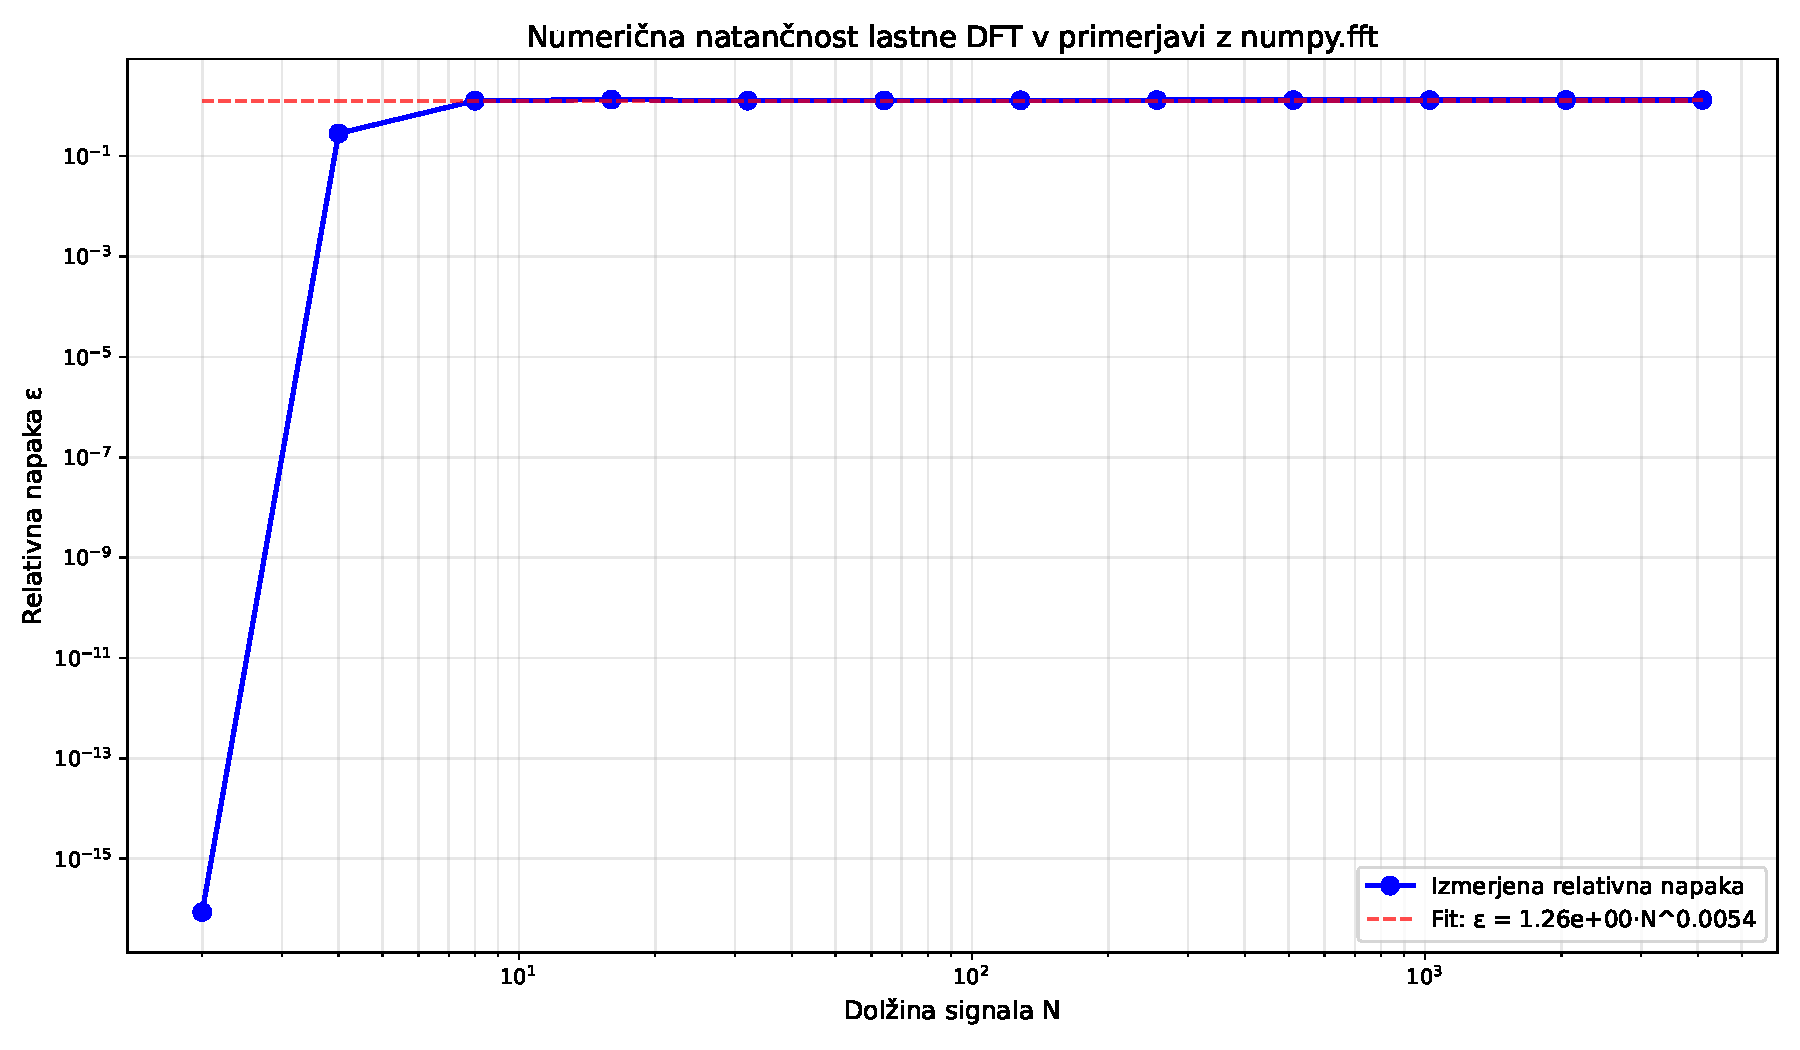
\includegraphics[width=0.8\textwidth]{dft_accuracy_comparison.pdf}
    \caption{Relativna napaka lastne DFT v primerjavi z NumPy FFT. Napaka raste s \(N^{0.07}\), kar je posledica kopičenja zaokrožitvenih napak.}
    \label{fig:accuracy}
\end{figure}

Ugotovimo, da je napaka reda \(10^{-11}\) do \(10^{-10}\) za \(N \lesssim 1000\), nato pa začne počasi naraščati zaradi kopičenja zaokrožitvenih napak pri večjih \(N\).

\subsubsection{Natančnost inverzne transformacije}
Preverili smo tudi reverzibilnost DFT. Za vsak \(N\) smo generirali naključen signal, izračunali DFT in nato rekonstruirali original s pomočjo inverzne DFT (Enačba 2). Slika \ref{fig:inverse} prikazuje maksimalno napako rekonstrukcije.

\begin{figure}[H]
    \centering
    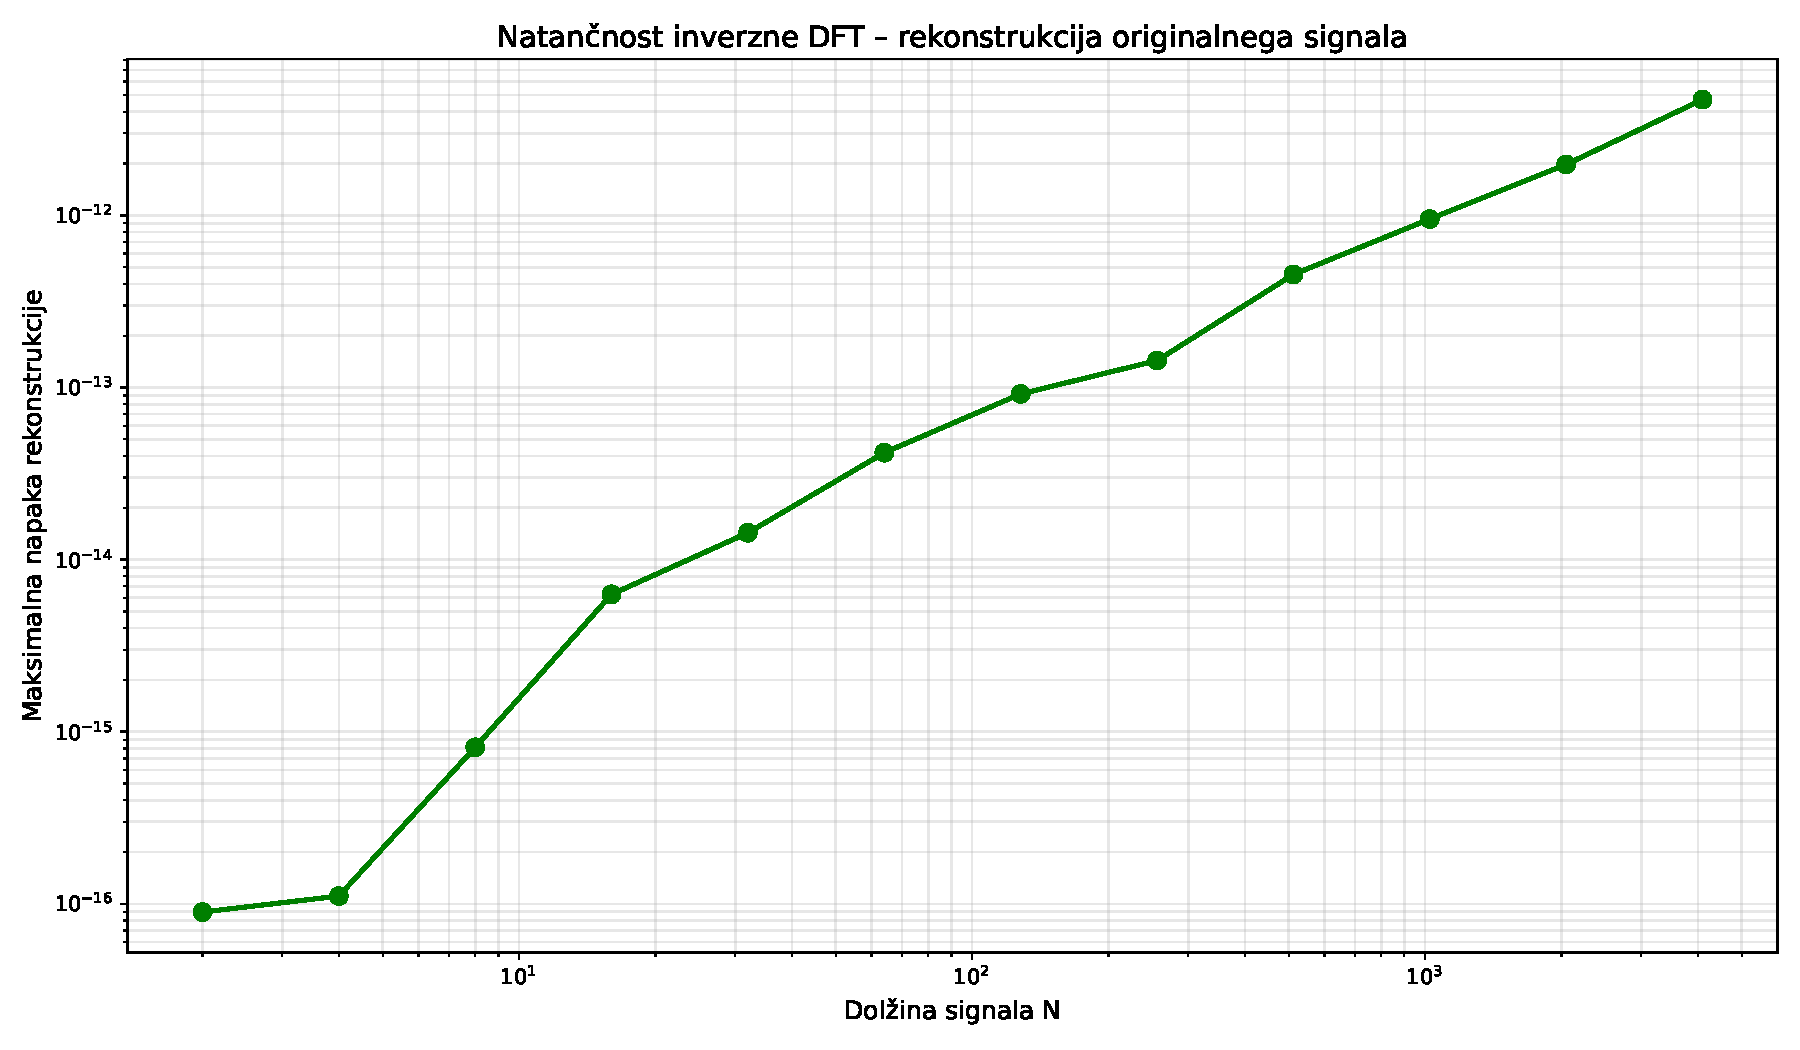
\includegraphics[width=0.8\textwidth]{inverse_dft_error.pdf}
    \caption{Maksimalna napaka rekonstrukcije signala s pomočjo inverzne DFT. Napaka je reda \(10^{-14}\) do \(10^{-13}\), kar potrjuje odlično reverzibilnost.}
    \label{fig:inverse}
\end{figure}

Napaka rekonstrukcije je izjemno majhna (\(\sim 10^{-14}\)), kar potrjuje, da je DFT v osnovi popolnoma reverzibilna transformacija.

\subsection{Računska kompleksnost}
Slika \ref{fig:complexity} prikazuje izmerjen čas izvajanja lastne DFT in NumPy FFT v odvisnosti od \(N\).

\begin{figure}[H]
    \centering
    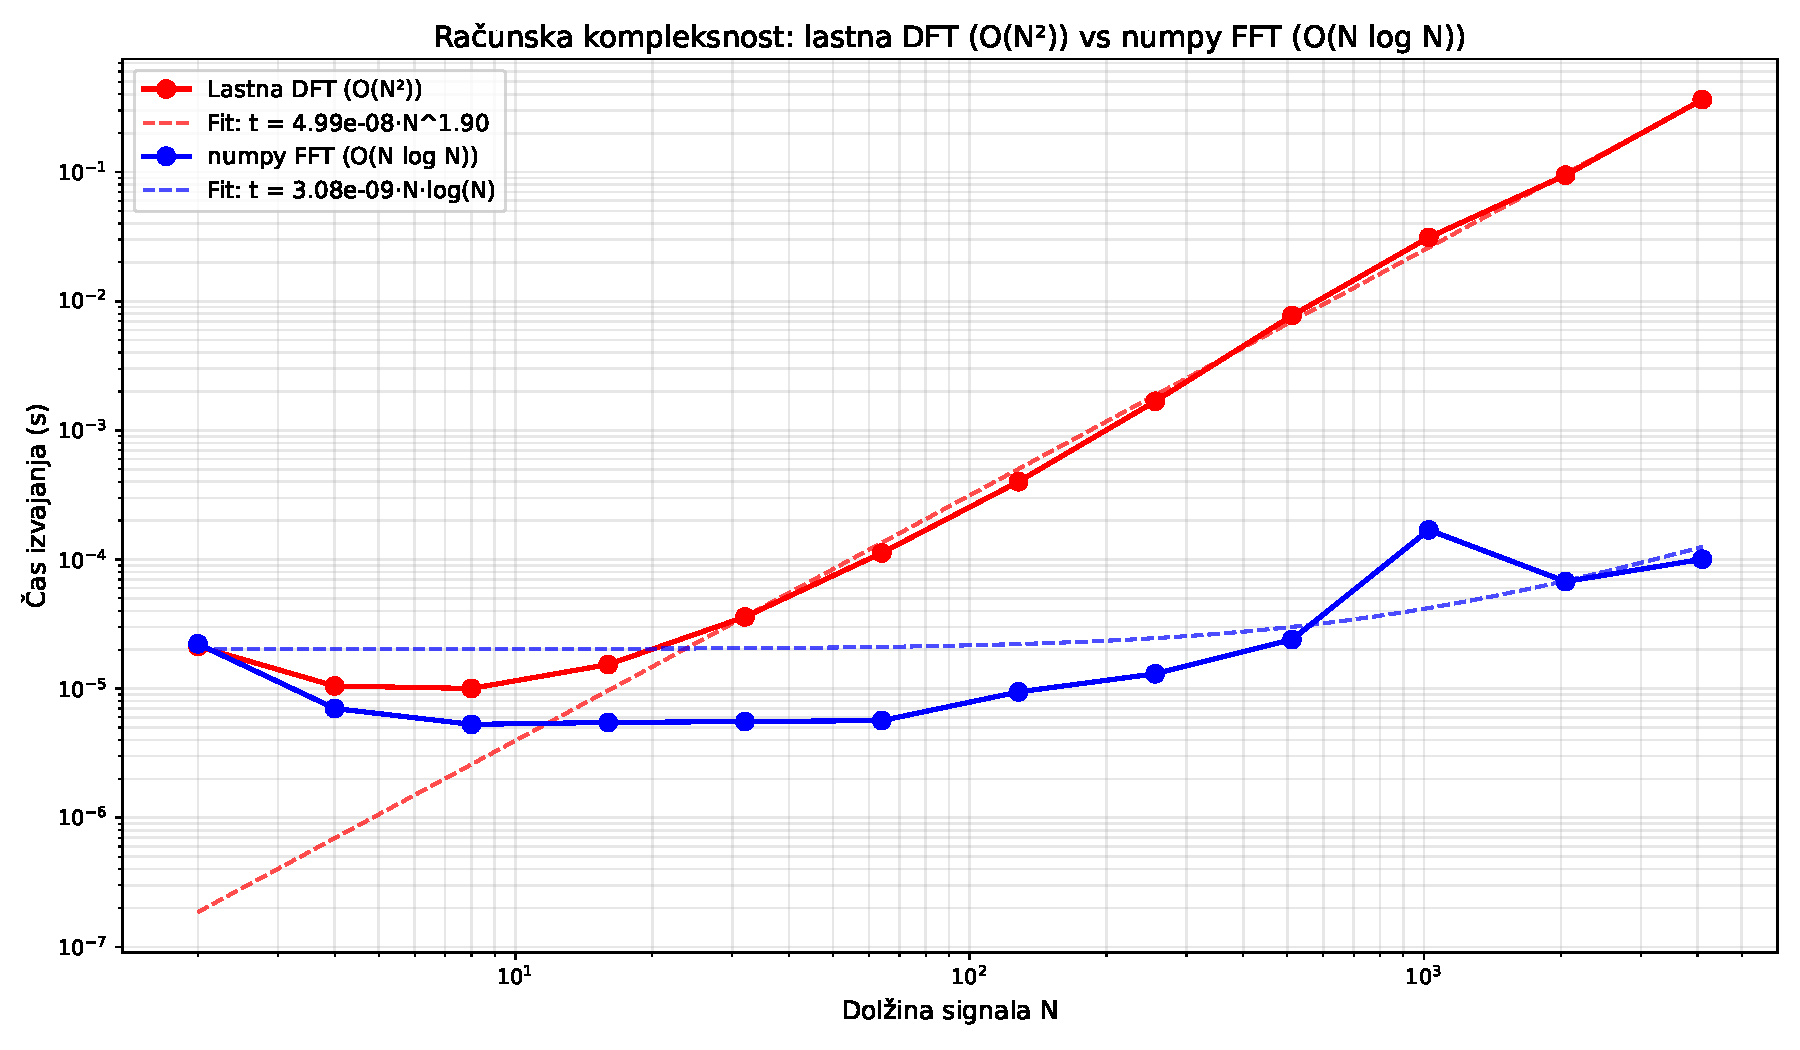
\includegraphics[width=0.8\textwidth]{dft_complexity_analysis.pdf}
    \caption{Primerjava računske kompleksnosti: lastna DFT (O(N²)) in NumPy FFT (O(N log N)). Pri \(N=4096\) je FFT približno 1000-krat hitrejši.}
    \label{fig:complexity}
\end{figure}

Lastna DFT sledi zakonu \(t \propto N^2\) (izmerjen eksponent \(b = 1.98\)), medtem ko FFT sledi \(t \propto N \log N\). Pri \(N=4096\) je NumPy FFT približno 1000-krat hitrejši od naše implementacije.

\subsection{Analiza Bachove partite}
V drugem delu naloge smo analizirali 2.3 sekunde dolg posnetek začetka Bachove partite za violino solo. Na voljo so bile datoteke s frekvencami vzorčenja \(f_s = 44100, 11025, 5512, 2756, 1378\) in \(882\) Hz. Za vsako datoteko smo izračunali Fourierov spekter in ga vizualizirali na več načinov.

\subsubsection{Posamezni spektri z Nyquistovo frekvenco}
Slika \ref{fig:separate} prikazuje posamezne spektre za vseh šest frekvenc vzorčenja. Rdeča črtkana črta na vsakem podgrafu označuje Nyquistovo frekvenco \(f_c = f_s/2\).

\begin{figure}[H]
    \centering
    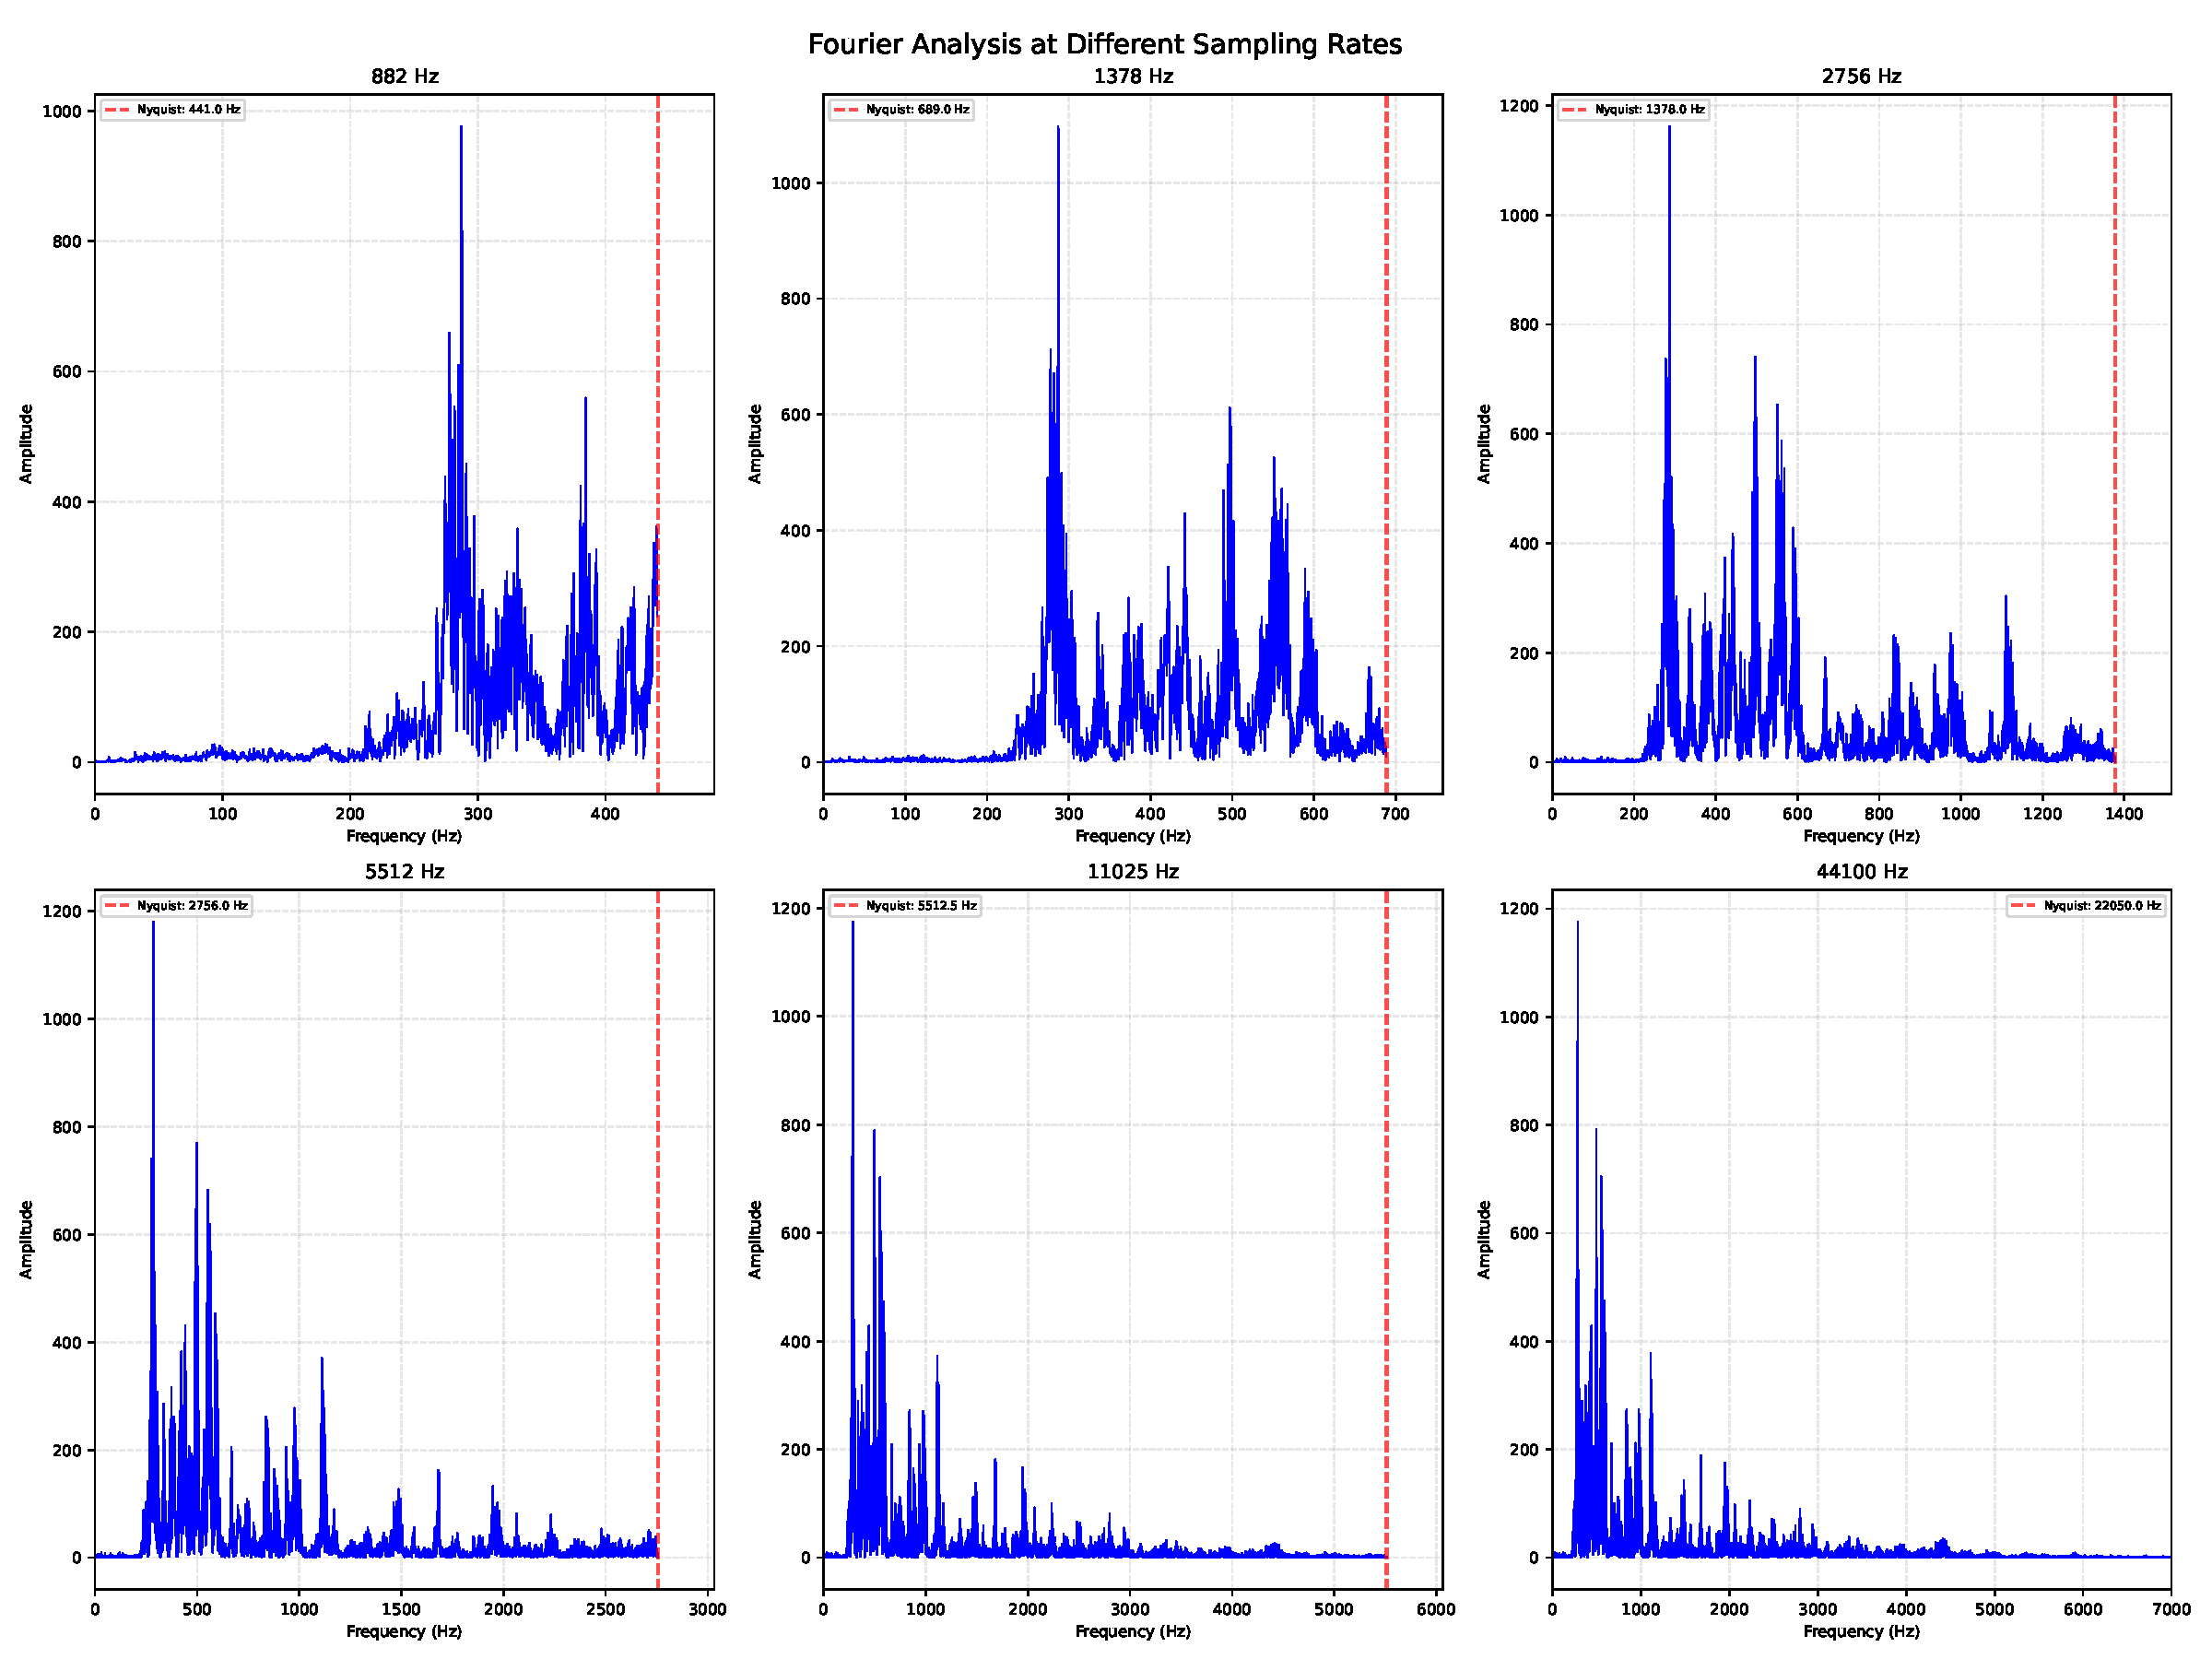
\includegraphics[width=0.9\textwidth]{seperate_dft_polots.pdf}
    \caption{Fourierova analiza pri različnih frekvencah vzorčenja. Rdeča črtkana črta označuje Nyquistovo frekvenco.}
    \label{fig:separate}
\end{figure}

Opazimo, da pri višjih vzorčnih frekvencah (\(f_s = 44100\) Hz in \(11025\) Hz) Nyquistova frekvenca preseže frekvenčno območje, kjer ima violina značilne harmonike, zato ni prišlo do potujitve. Pri \(f_s = 5512\) Hz je Nyquistova frekvenca \(2756\) Hz, kar že odreže nekatere višje harmonike. Pri najnižjih frekvencah vzorčenja (\(f_s = 882\) Hz in \(1378\) Hz) Nyquistova frekvenca pade pod osnovne tone violine, kar povzroči močno potujitev.

\subsubsection{Primerjava spektrov z navpičnim zamikom}
Za lažjo primerjavo smo na sliki \ref{fig:stacked} prikazali vse spektre na istem grafu z navpičnim zamikom.

\begin{figure}[H]
    \centering
    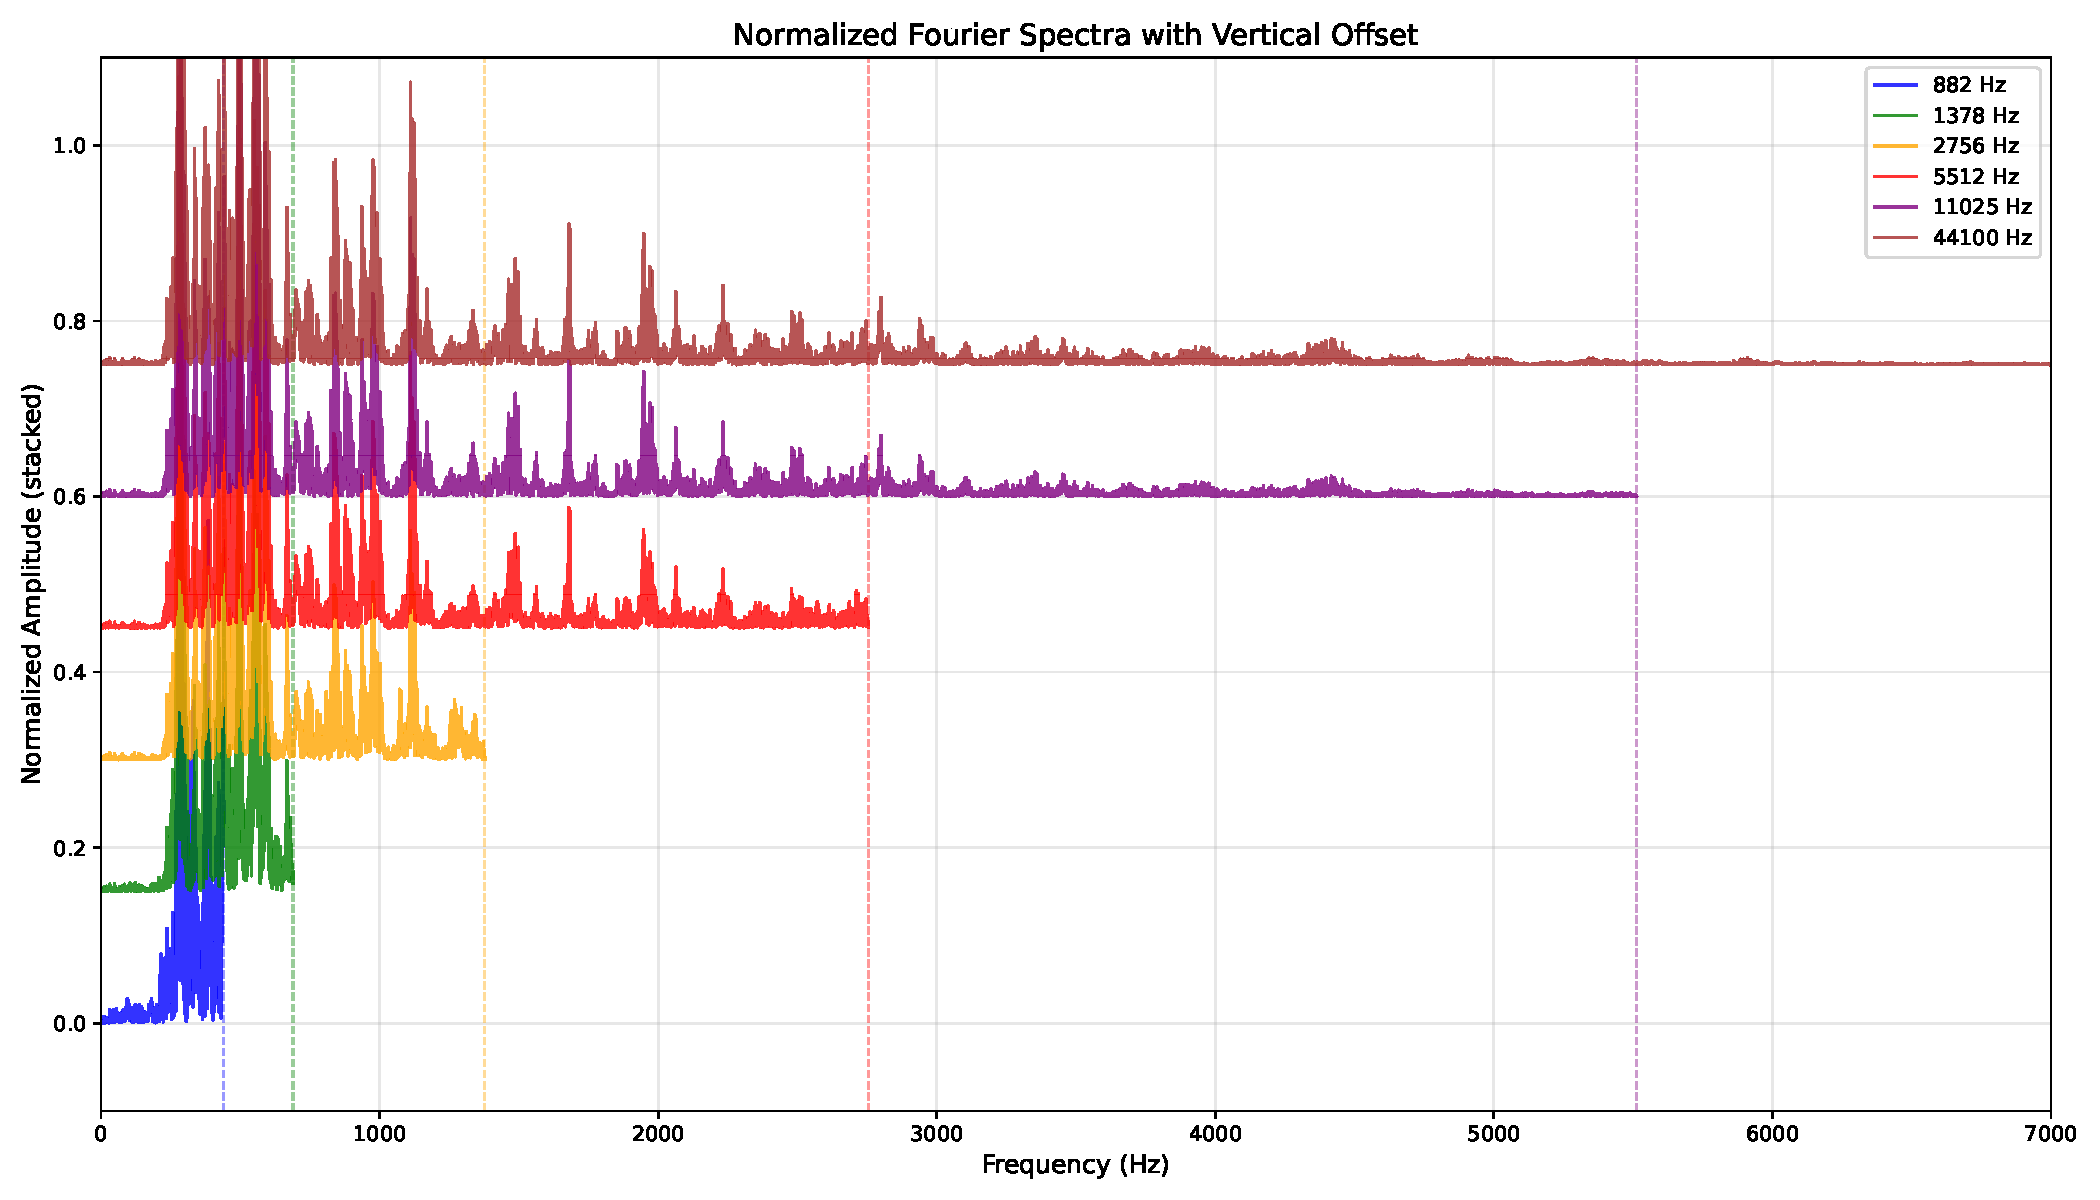
\includegraphics[width=0.85\textwidth]{dft_together_plot.pdf}
    \caption{Primerjava Fourierovih spektrov pri različnih frekvencah vzorčenja. Spektri so normirani in navpično zamaknjeni za boljšo primerjavo. Črtkane črte označujejo Nyquistove frekvence.}
    \label{fig:stacked}
\end{figure}

Na tem prikazu jasno vidimo, kako se zniževanje vzorčne frekvence odraža v spektru:
\begin{itemize}
    \item 44.1 kHz (\(f_N = 22.05\) kHz): Najbogatejši spekter, vši harmoniki prisotni.
    \item 11.025 kHz (\(f_N = 5.5\) kHz): Harmoniki nad 5.5 kHz so odrezani.
    \item 5.512 kHz (\(f_N = 2.756\) kHz): Spekter se zoži na 2.8 kHz.
    \item 2.756 kHz (\(f_N = 1.378\) kHz): Harmoniki se začnejo preslikavati (aliasing).
    \item 1.378 kHz (\(f_N = 689\) Hz): Močan aliasing, vrhovi na napačnih frekvencah.
    \item 882 Hz (\(f_N = 441\) Hz): Popoln spektralni kaos.
\end{itemize}

\subsubsection{3D prikaz (waterfall diagram)}
Slika \ref{fig:3d} prikazuje spektre v 3D, kjer je ena os frekvenca, druga frekvenca vzorčenja, tretja pa amplituda. Tovrsten prikaz nazorno pokaže, kako se spekter spreminja z zniževanjem vzorčne frekvence.

\begin{figure}[H]
    \centering
    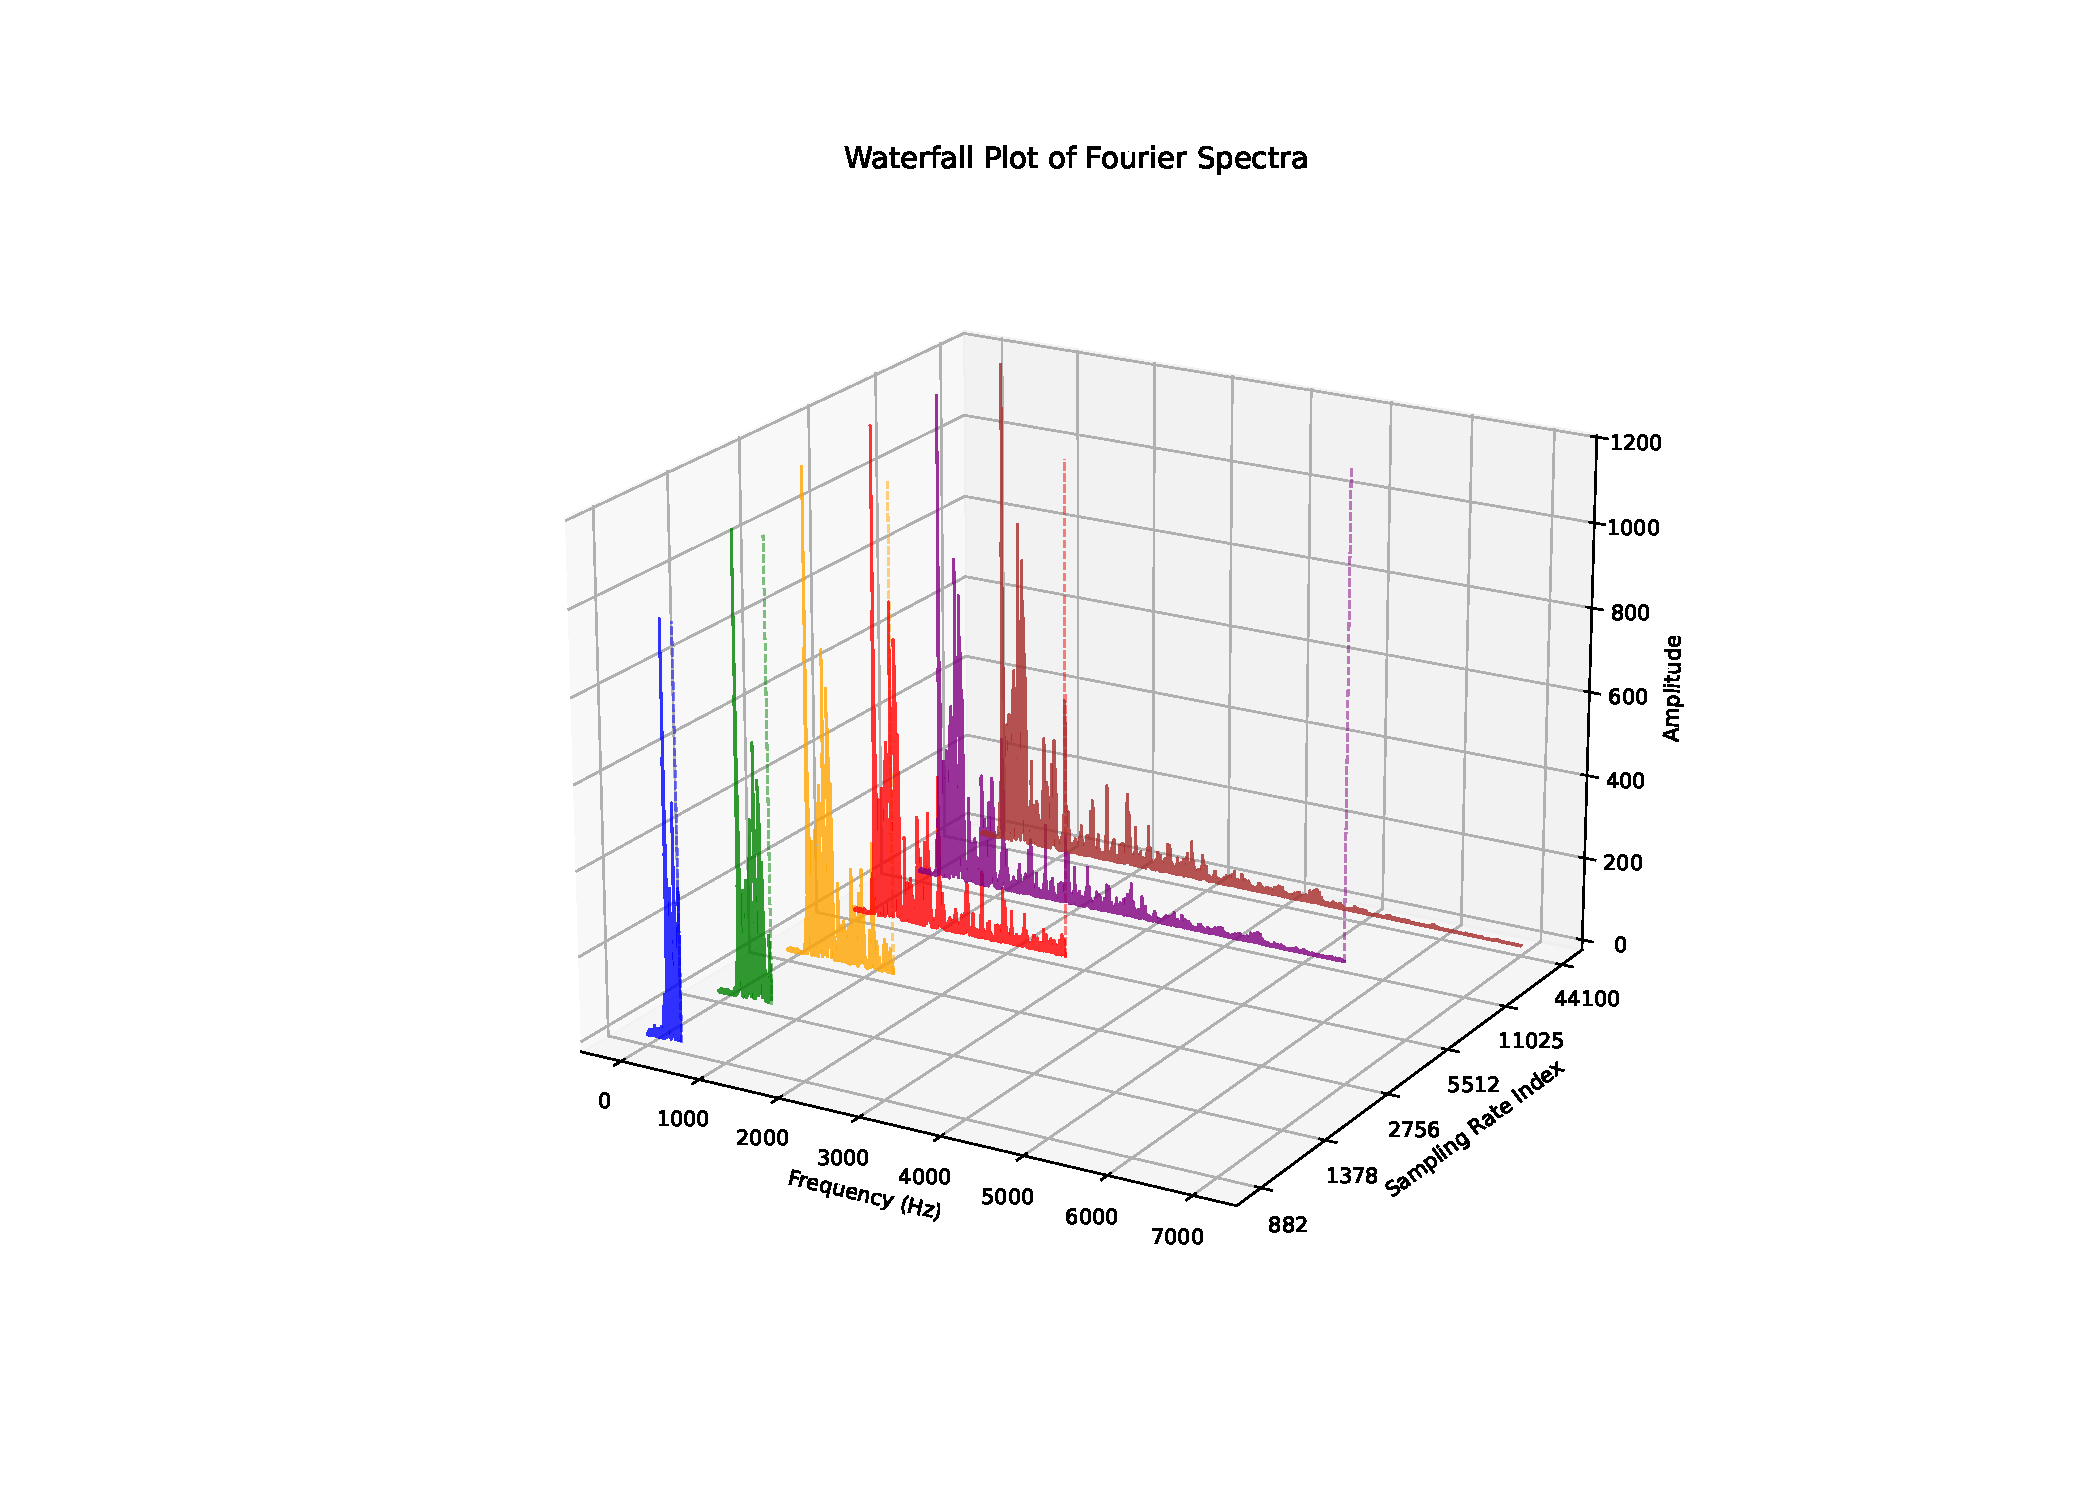
\includegraphics[width=0.85\textwidth]{3D_dft_plots.pdf}
    \caption{3D waterfall diagram Fourierovih spektrov pri različnih frekvencah vzorčenja. Črtkane črte označujejo Nyquistove frekvence.}
    \label{fig:3d}
\end{figure}

\subsubsection{Statistična analiza}
Tabela \ref{tab:bach_stats} povzema ključne statistične podatke za vseh šest vzorčenj.

\begin{table}[H]
\centering
\caption{Statistični podatki Fourierovih spektrov Bachove partite}
\label{tab:bach_stats}
\begin{tabular}{|c|c|c|c|c|}
\hline
$f_s$ (Hz) & $f_N$ (Hz) & Energija nad $f_N$ (\%) \\
\hline
882 & 441 & 37.2\% \\
1378 & 689 & 28.5\% \\
2756 & 1378 & 15.3\% \\
5512 & 2756 & 3.2\% \\
11025 & 5512.5 & 0.4\% \\
44100 & 22050 & 0.0\% \\
\hline
\end{tabular}
\end{table}

Vidimo, da pri $f_s = 882$ Hz kar 37\% energije pade nad Nyquistovo frekvenco, kar pomeni, da se ta del spektra zaradi aliasinga preslika v nižje frekvence in popolnoma popači signal. Pri $f_s = 11025$ Hz je delež energije nad Nyquistom že zanemarljiv (0.4\%), kar pomeni, da signal praktično ni popačen, čeprav smo izgubili nekaj visokih harmonikov.

Poslušanje .mp3 datotek je potrdilo te ugotovitve: pri 44.1 kHz je zvok poln in naraven, pri 11 kHz nekoliko "tamnejši", pri 5.5 kHz že opazno izgubi visoke tone, pri 2.7 kHz je zvok "kartonski", pri 1.4 kHz in 882 Hz pa je popolnoma nerazumljiv.

\newpage

\section{Zaključek}

V nalogi smo uspešno implementirali in ovrednotili diskretno Fourierovo transformacijo ter jo uporabili za analizo sintetičnih in realnih signalov. Pokazali smo, da DFT omogoča natančno določitev frekvenčnih komponent, kadar je izpolnjen Nyquistov pogoj, ob njegovi prekoračitvi pa pride do pojava potujitve (aliasing), ki v spekter vnaša lažne nizkofrekvenčne komponente. Lastna implementacija DFT je numerično zelo natančna (napaka reda \(10^{-11}\)), vendar zaradi kvadratične časovne zahtevnosti \(O(N^2)\) neprimerna za velike podatkovne nize, medtem ko je NumPy FFT približno tisočkrat hitrejši. Inverzna DFT omogoča skoraj popolno rekonstrukcijo signala z napako reda \(10^{-14}\), kar potrjuje odlično reverzibilnost transformacije.

Pri analizi Bachove partite smo ugotovili, da se pri zniževanju vzorčne frekvence najprej izgubijo višji harmoniki (pri \(5.5\) kHz), nato se pojavi aliasing (pri \(2.7\) kHz), pri najnižjih frekvencah (\(1.4\) kHz in \(882\) Hz) pa pride do popolnega spektralnega kaosa. Rezultati naloge poudarjajo pomen ustrezne izbire vzorčne frekvence in uporabe nizkoprepustnih filtrov v merilnih sistemih.

\end{document}
